\chapter{Implementace} 
\section{Architektura}
V tomto frameworku \cite{framework} rozlišujeme klientskou a serverovou část. Serverová část generuje data pro klienta a tímto způsobem ovlivňuje ovládací prvky, které klientská část aplikace zobrazuje uživateli. Diagram nasazení na obrázku \ref{img:deploymentFrameworkDiagram} zachycuje použití frameworku. Serverová část frameworku je nasazena na serveru a je schopná generovat definice formulářů s použitím frameworku AspectFaces \cite{aspectFaces}. Tyto definice jsou převedeny na model, který je možné upravit a odeslat klientovi. Aby byla tato část plně funkční, je potřeba nasadit aplikaci na aplikační server na platformě Java EE. Nicméně v případě využití pouze staticky generovaných definic lze aplikaci nasadit na libovolný aplikační server, který bude poskytovat klientům definice kompatibilní s definici poskytovanými při dynamickém generování. Specifikace komponenty, je poté zaslána na klienta, který ji interpretuje za použití klientské části zvané AFSwinx. Tato část využívá i serverovou část, a to z důvodu kompatibilnosti objektů a jejich vlastností. Přidání do projektu lze provést tak, že se do adresáře s knihovnami, obvykle bývá nazván lib, vloží přeložený jar soubor nebo se přidá projekt jako Maven závislost. Maven \cite{maven} je framework pro správu projektů, sloužící k buildu aplikací, dokumentací a spouštění testů. Pomocí Mavenu lze do projektu vkládat závislosti na dalších knihovnách. V současné době není framework k dispozici v centrálním repositáři, a proto je potřeba stáhnout aktuální verzi a zkompilovat ji do lokálního repositáře. 
\subsection{Server}
Jak již bylo zmíněno, server využívá ke generování serverovou část frameworku nazvanou AFRest. Na obrázku \ref{img:serverSide} jsou zobrazeny třídy a balíčky, které tato část využívá. Jsou zde výčtové typy, které určují podporované komponenty a jejich vlastnosti, dále objekty zodpovědné za informace o volbě layoutu a objekty nesoucí informace o definicích, na jejichž základě budou sestaveny formuláře či tabulky klientem a samozřejmě třídy zodpovědné za inspekci dat. Framework doplňuje do AspectFaces několik anotací, které lze využít při generování definic. Jsou to následující anotace:
\begin{enumerate}
\item @UIWidgeType - tato anotace určuje typ widgetu, který bude využit. Do XML šablon, které se používají při generování definic, je propagována jako proměnná s názvem widgetType
\item @UILayout - tato anotace definuje layout na dané proměnné. Lze specifikovat typ layoutu, jeho orientace a pozice popisu prvku. Do XML šablon jsou tyto hodnoty propagovány jako proměnné layout, layoutOrientation a labelPossition. 
\end{enumerate}
Výše zmíněné anotace akceptují pouze hodnoty z výčtových typů v balíčku common. V případě typu komponenty, neboli widgetType, přijímá anotace hodnoty ze třídy SupportedWidgets. V případě anotace určující layout lze vložit pouze hodnoty z výčtových typů LayoutDefinitions, LayoutOrientation a LabelPosition. Hlavní výhodou tohoto řešení, je typová kontrola a jistota, že klient obdrží od serveru pouze takové hodnoty, s kterými je schopný pracovat. Stejným principem jsou řešeny validace a proměnné, které definují vlastnosti jednotlivých komponent. 

\subsubsection{Generování modelu}
Výsledkem inspekce objektu je model, který nese informace potřebné k tomu, aby klient mohl sestavit formulář či tabulku a byl do těchto komponent schopný vložit data získaná ze serveru. Na obrázku \ref{img:finalModel} je konečná podoba modelu vytvořeného k tomuto účelu. Model je výsledkem hledání analytických tříd z doménového modelu na obrázku \ref{img:metadataModel}. Tento model byl popsán již v analytické části, nicméně v této části je model kompletní, a proto zde budou uvedeny pouze změny oproti původnímu modelu. Proměnné, které nesou informace o layoutu, typu komponenty validátorech a jejich typech jsou výčtové typy. Jak již bylo zmíněno výhodou je typová bezpečnost a jednoznačnost vlastností, které framework podporuje. Model slouží také jako fasáda k nastavení dodatečných atributů. Jedním z těchto atributů je proměnná options ve třídě AFFieldInfo. Tato proměnná drží informace o možných hodnotách, kterých může komponenta nabývat. V současné verzi je tento atribut využit u komponent výběrového typu, mezi které patří například zaškrtávací políčka či výběrová menu. Programátor specifikuje množinu těchto hodnot, ve které klíč určuje hodnotu, jež bude odeslána na server. Text, který bude zobrazen uživateli je určen proměnnou value. Tyto možnosti nejsou generovány automaticky a v případě potřeby je musí programátor specifikovat ručně. A to tak, že určí množinu dat a pole, ke kterému je přiřazeno. Třída AFMetaModelPack zapouzdřuje způsob jakým se množina dat nastaví na konkrétní políčko a nabízí uživateli funkci, která je schopná nastavení provést na základě dat, zadaných uživatelem.

K dynamickému generování definic se využívá framework AspectFaces \cite{aspectFaces}, který umožňuje na základě mapování rozhodnout, jaká komponenta bude použita pro konkrétní proměnnou dané třídy. Dále nabízí určení layoutu, jež bude použit, a samozřejmě určení mapovacího souboru. Tímto lze docílit mnoha různých transformací. Tento framework je potřeba nejprve nastavit, nicméně toto nastavení provede za vývojáře serverová část frameworku AFRest. Rozhraní AFRest z obrázku \ref{img:finalModel} a jeho implementace AFRestGenerator provedou kompletní nastavení a spustí generování dat. Rozhraní umožňuje uživateli určit mapovací soubor a šablonu, která bude použita. Mapování lze použít na všechny proměnné objektu, či může vývojář určit, které mapování se použije na konkrétní proměnnou. Ukázka mapování z frameworku AspectFaces je znázorněna v ukázce zdrojových kódu \ref{code:xmlMapping}. Proměnná typu String se bude mapovat na vstupní textové pole, které je definováno v structure/inputField.xml. V případě, že se bude jednat o typ password, bude se proměnná typu String mapovat na vstupní textové pole typu, které místo vepsaných znaků zobrazuje zástupné znaky. Komponenta je definována v structure/inputPassword.xml. Typ Address, což je neprimitivní datový typ se bude mapovat na entitní typ, jehož definice je v structure/entity.xml.
\begin{lstlisting}[caption=Ukázka mapování proměnných na komponenty,
label={code:xmlMapping}, basicstyle=\footnotesize]
<mapping>
	<type>String</type>
	<default tag="structure/inputField.xml" maxLength="255"/>
	<condition expression="${type == 'password'}" tag="structure/inputPassword.xml" />
</mapping>
<mapping>
	<type>Address</type>
	<default tag="structure/entity.xml" />
</mapping>
\end{lstlisting}

Mapování tedy určí soubor s komponentou, který bude reprezentovat aktuální proměnnou. Soubor s definicí komponenty je pak dále využit k finální definici proměnné. Ukázka vstupního textového pole je v ukázce zdrojových kódu \ref{code:xmlInputField}. Komponenta je v kořenovém elementu widget. Jelikož se jedná pouze o fragment xml, který je použit ke složení celé definice, jenž je uvedena v příloze v ukázce zdrojových kódů \ref{code:xmlCompleteDefinition}, není zde uvedena deklarace XML \cite{xml}. Ve výsledném XML již však deklarace uvedena je. Popis jednotlivých uzlů je v tabulce \ref{table:xmlComponentAttributes}.

\begin{lstlisting}[caption=Ukázka definice komponenty,
label={code:xmlInputField}, basicstyle=\footnotesize]
<widget>
	<widgetType>textField</widgetType>
	<fieldName>$field$</fieldName>
	<label>$label$</label>
	<validations>
		<required>$required$</required>
		<minLength>$minLength$</minLength>
		<maxLength>$maxLength$</maxLength>
	</validations>
	<fieldLayout>
		<layoutOrientation>$layoutOrientation$</layoutOrientation>
		<labelPossition>$labelPossition$</labelPossition>
		<layout>$layout$</layout>
	</fieldLayout>
</widget>
\end{lstlisting}
Knihovna AspectFaces umožňuje určovat způsob, jakým bude prováděna inspekce. Tento způsob se určuje v šablonách. K optimálnímu využití je nejvýhodnější použít způsob, při kterém je provedena inspekce všech proměnných, které mají definováno mapování. V případě jednoduchých datových typů je vše v pořádku. Nicméně knihovna neobsahovala nativní podporu pro neprimitivních datových typů a v případě, že byla použita inspekce, která by nevyužívala JSF, nebyla by provedena inspekce složitých datových typů. Z tohoto důvodu je důležité, aby se všechny neprimitivní datové typy mapovali na entity.xml, která je znázorněna v části zdrojového kódu \ref{code:xmlEntity}. Framework totiž pro všechny tyto entity provede inspekci znovu, následně části sestaví a tím vznikne kompletní definice. V tomto bodě lze určit mapování a šablony, které se mají při rekurzivní inspekci použít. Framework AspectFaces byl proto doplněn o proměnné, které umí vrátit kanonický název třídy a na základě tohoto názvu lze provést nad touto třídou inspekci. Jak je patrné z výsledné definice, každý uzel má svého rodiče. Na základě rodiče lze jednoznačně určit, kam uzel patří. Tato vlastnost umožňuje provádět inspekci i nad třídami, které mají více proměnných stejného datového typu. Klient totiž potřebuje znát strukturu objektu, aby ho mohl zpětně sestavit a odeslat zpět na server, který objekt přijme. Znalost struktury klient taktéž vyžaduje v případě získávání dat.
\begin{lstlisting}[caption=Ukázka definice neprimitivního datového typu,
label={code:xmlEntity}]
<entityClass>
	<entityFieldType>$DataTypeFullClassName$</entityFieldType>
	<fieldName>$fieldName$</fieldName>
</entityClass>
\end{lstlisting}

\begin{table}[width=\linewidth]
\begin{center}
\caption{Uzly XML, které definují strukturu dat}
\label{table:xmlComponentAttributes}
\begin{tabular}{|p{7cm}|p{7cm}|}
\hline
\textbf{Uzel} & \textbf{Popis} \\
\hline
widget & 
Typ komponenty. Určuje, jak komponentu bude klient interpretovat. \\
\hline
fieldName &
Název aktuální proměnné, kterou komponenta zastupuje. \\
\hline
Label &
Popis komponenty, který bude zobrazen uživateli. \\
\hline
validations &
Validace, které budou umět komponenta ověřit. \\
\hline
fieldLayout&
Popis layoutu, který bude na komponentě použit. \\
\hline
\end{tabular}
\end{center}
\end{table}

\subsubsection{Použití}
Aby byl klient schopný získat definice dat, musí serverová strana poskytovat zdroj těchto definic. V tomto zdroji server využije serverovou část frameworku ke generování dat. Použití je přímočaré a ukázka zdroje je zobrazena v části zdrojového kódu \ref{code:serverDefinition}. Nejprve je vytvořena instance třídy AFrestGenerator, která umožňuje generování dat, jenž jsou následně odeslána klientovi. Generátor nastaví framework AspectFaces automaticky, nicméně očekává, že bude framework AspectFaces použit. Ke správnému použití je potřeba, aby ve WEB-INF byly konfigurační soubory a aby existovali mapovací soubory a definice komponent. V tomto případě využije implicitního nastavení pro mapování i šablony. Bude použito mapování v souboru structure.config.xml a šablona v template/structure.xml. Tyto ukázkové soubory jsou poskytovány spolu s frameworkem.

Zdroj poskytuje definice dat. V případě, že klient požaduje data do vygenerované definice, je potřeba poskytnout mu objekt stejného typu, nad kterým byla prováděna definice, nebo objekt se stejnými proměnnými a datovými typy. V tomto případě třídu Country. Klientská strana nerozlišuje datový typ obdrženého objektu, avšak očekává, že objekt bude mít určité proměnné, ke kterým se budou vázat specifické validace. V některých případech je žádoucí, aby se na úrovni business a view nepracovalo s databázovou entitou, ale s jejím mapovacím objektem. V části zdrojových kódů \ref{code:serverData} je příklad získání dat do již vygenerovaného formuláře či tabulky. Zdroj využije EJB \cite{javaEE} managera CountryManager k získání konkrétní instance třídy Country z databáze. Tuto instanci vrátí klientovi. Tento zdroj nemá žádnou vazbu na předchozí zdroj, který generoval definice. Vývojář tedy v případě použití frameworku nemusí měnit stávající implementaci, pokud již nějaká existuje. Stejně tak nemá použití frameworku dopad na klienty, kteří již používají webové API serveru. Zodpovědnost za správnou interpretaci dat je na klientské straně.
\begin{lstlisting}[caption=Zdroj poskytující konkrétní instanci třídy Country,
label={code:serverData}, basicstyle=\footnotesize]
@GET
@Path("/{id}")
@Produces({MediaType.APPLICATION_JSON})
@Consumes({MediaType.APPLICATION_JSON})
public Response getCountry(@PathParam("id") int id) {
	try {
		CountryManager<Country> countryManager = getCountryManager();
		Country country = countryManager.findById(id);
		return Response.status(Response.Status.OK).entity(country).build();
	} catch (BusinessException e) {
		return Response.status(Response.Status.BAD_REQUEST).build();
	} catch (NamingException e) {
		return Response.status(Response.Status.INTERNAL_SERVER_ERROR).build();
	}
}
\end{lstlisting}

\subsection{Klient}
Klientská část aplikace, využívá klientskou část frameworku ke generování formulářů či tabulek. Definice a data získává ze serveru. Referenční implementace je napsána pro aplikace na platformě JavaSE, které získávají data ze serveru a k vizualizaci využívají technologie Swing. Integrace frameworku do klientské aplikace je možná dvěma způsoby. Prvním z nich je vložení knihovny do složky lib a druhým je přidání Maven \cite{maven} závislosti. 
\subsubsection{Komponenty}
Klientská část umožňuje generovat tabulky nebo formuláře. Tyto celky označujeme jako komponenty. V případě formuláře se tato komponenta skládá z dalších aktivních ovládacích prvků. Komponenty jsou děděny z třídy AFSwinxTopLevelComponent, která implementuje rozhraní AFSwinxInteraction, jež vynucuje implementovat metody k získání modelu dat a k jejich odeslání zpět na server. Součástí je také validace dat. Mimo výše zmíněné rozhraní implementuje třída ještě rozhraní ComponentResealization. Toto rozhraní je využito k zpětnému získání dat z komponent. Aby bylo možné přidávat komponenty do již existující aplikace, tak tato komponenta ještě dědí od třídy JPanel, což zajistí, že výslednou komponentu lze přidat na jakékoliv místo ve stávající Swingové aplikaci. Vývojář může nad takto generovanými komponentami provádět operace. V případě odeslání dat na server lze tuto akci vyvolat metodou sendData. Komponenta již sama provede validaci dat, sestavení dat a jejich odeslání.

Při návrhu jsem se zaměřil i na použitelnost, neboť je potřeba aby framework umožňoval dodatečná nastavení. Nicméně pokud se vývojář bude s frameworkem učit, je velice pravděpodobné, že bude chtít vytvořit první prototyp, aby si vyzkoušel funkčnost. Z tohoto důvodu byla zavedena třída AFSwinx, která slouží jako správce komponent. Třída je singleton \cite{gamma} a slouží jako fasáda \cite{gamma}pro ovládání frameworku.  Umožňuje komponenty vytvářet, přidávat, mazat a nastavovat globální skin a lokalizace. Důležitou součástí je i získání již sestavené komponenty. Každá komponenta je jednoznačně určena svým identifikátorem, který si vývojář zvolí. Na základě tohoto identifikátoru je zaregistrována a lze k ní získat přístup a provádět nad ní operace. Vzhled jednotlivých prvků v komponentě již není možné po vygenerování měnit. Skiny a lokalizace musí být tedy nastaveny před samotným vygenerováním. Také je potřeba určit způsoby připojení ke zdrojům a jejich URI. Proces vytváření komponent vyžaduje několik operací, které na sebe navazují. V případě, že by byl tento proces ponechán na vývojáři, byl by framework nepoužitelný. Z tohoto důvodu poskytuje třída AFSwinx buildery \cite{gamma} pro tabulky a formuláře, které komponenty sestaví, vloží do nich data a vývojáři vrátí výsledný JPanel. Typ komponenty určuje vývojář a buildery umí vytvořit formulář či tabulku na základě jedné definice. V případě tabulky je možné ještě provést dodatečné nastavení. Jedná se o automatické nastavení šířky sloupečků a nastavení velikosti tabulky. Ukázka vytvoření formuláře je zobrazena v části zdrojových kódů \ref{code:formGeneration}. Nejprve je potřeba získat instanci builderu, který bude použit. Typ builderu určí, zdali bude vytvořena tabulka či formulář. V tomto konkrétním případě bude vytvořen formulář. Metamodel získává klient ze serveru. Framework zapouzdřuje způsob získání dat, vývojář tedy musí definovat pouze zdroje. Jednou z možností je specifikovat zdroje jako samostatné objekty, druhou možností je využít XML. V případě použití XML souboru musí být uveden soubor a identifikátor připojení. Tyto vlastnosti jsou nastaveny builderu pomocí metody initBuilder, která očekává identifikátor formuláře, soubor se specifikací připojení a identifikátor připojení. Builder má samozřejmě několik přetížených metod initBuilder. Tímto lze docílit různých způsobů počátečního nastavení. Metoda buildComponent již vygeneruje výsledný formulář. Pokud se při generování vyskytne chyba, pak je vyhozena výjimka AFSwinxBuildException. Je na vývojáři jak výjimku zpracuje. V ukázce \ref{code:formGeneration} je zobrazen dialog s chybovým hlášením.

\begin{lstlisting}[caption={Generování formuláře na klientovi},
label={code:formGeneration}, basicstyle=\footnotesize]
InputStream connectionResrouce = getClass().getClassLoader().getResourceAsStream("connection.xml");
try {
	AFSwinxForm form =
		AFSwinx.getInstance().getFormBuilder()
		.initBuilder(loginFormName, connectionResrouce, "loginForm")
		.buildComponent();
} catch (AFSwinxBuildException e) {
	getDialogs().failed("afswinx.build.title.failed", "afswinx.build.text.failed", e.getMessage());
}
\end{lstlisting}

\section{Přenos modelu server klient a generování komponent}
Model, na jehož základě jsou generovány komponenty, je přenášen ze serveru na klienta. Klient musí tento model správně zpracovat a interpretovat. Nejprve je však potřeba model získat. Pro přenos modelu je použit protokol HTTP či HTTPS. Klientská strana poskytuje vývojáři nativní podporu k získání dat ze serveru. K tomuto účelu je využit framework HttpComponents \cite{apacheHttp}, který poskytuje předpřipravené komponenty, jež lze využít k vytváření HTTP či HTTPS požadavků. Využitím této knihovny se zjednoduší použití našeho frameworku, neboť vývojář nemusí ztrácet čas vytvářením tříd, které by byly schopné získat data ze serveru. Bohužel použití má i své nevýhody. Vývojář nemůže ovlivnit implementaci získání dat, pouze může ovlivnit způsob a to změnou ve specifikaci zdrojů a způsobů připojení. Z tohoto důvodu lze specifikovat zdroje ve formátu XML s podporou EL. K získání modelu je potřeba mít definovaný zdroj v uzlu metamodel. Uzel se specifikací konkrétních dat, a umístění, kam data odeslat je nepovinný. Zpracování pomocí DOM parseru je však provedeno nad všemi uzly konkrétního připojení a výsledkem je třída AFSwinxConnectionPack, která má reference na konkrétní připojení reprzentovanou třídou AFSwinxConnection. Ukázka je na obrázku \ref{img:connectionPack}. Mimo adresy, portu a protokolu lze specifikovat i hlavičku a v případě zabezpečení zdroje autorizaci k tomuto zdroji.

\begin{figure}[h!]
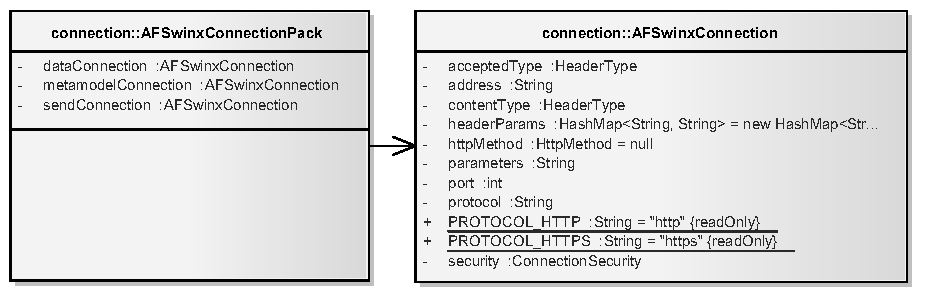
\includegraphics{images/connectionPack}
\caption{Třídy zodpovědné za specifikaci zdrojů a způsobu připojení.}
\label{img:connectionPack}
\end{figure}

\subsection{Generování komponent}
Vývojář na základě builderu určí, jaká komponenta se bude generovat. Sekvenční diagram je na obrázku \ref{img:sdDiagram}. Z diagramu je patrné, že builder nejprve získá model ze serveru na základě specifikace zdroje, který mu byl předán během inicializace. Od serveru získá klient třídy reprezentující metamodel. Tento metamodel byl již popsán a je na obrázku \ref{img:finalModel}. Klient nyní začne rekurzivně vytvářet již konkrétní aktivní prvky. Pro každou proměnnou objektu bude vygenerován widget. Pokud se jedná o neprimitivní datový typ, pak se k příslušnému typu vyhledá jeho reprezentace v metamodelu a generování bude pokračovat tímto objektem. Takovýto přístup zajišťuje zachování pořadí proměnných, které lze měnit na serverové straně, nikoliv však na klientovi. Typ aktivního prvku určuje atribut widgetType, který je součástí každého popisu konkrétní proměnné. Formulářový builder si nechá vytvořit od tovární třídy WidgetBuilderFactory, která je zodpovědná za vytváření konkrétního builderu, builder jenž je schopný vytvořit požadovaný aktivní prvek. Tento builder vrátí již konkrétní komponenty, jako jsou například vstupní textová pole, zaškrtávací políčka a další. Před kompletním generováním aktivního prvku lze nastavit jazykové lokalizace a skin. Tyto aktivní komponenty jsou zapouzdřeny v objektu AFSwinxPanel. Důvodem je, to že tento panel již zohledňuje layout dané komponenty a mimo aktivní prvek obsahuje i popis, placeholder určený k zobrazení validačního hlášení, a všechny validace, které musí být nad tímto prvkem vykonány. Panel si také udržuje jednoznačný identifikátor v rámci formuláře, na základě kterého lze určit, jakou proměnnou prvek reprezentuje a její umístění v hierarchii tříd. Panel je následně přidán do dalšího panelu, který udržuje všechny prvky formuláře. V rámci tohoto formulářového panelu jsou také zohledněny layouty a uspořádání komponent. V tomto bodě je formulář sestaven a lze již nad ním provádět validace, či je možné formulář odeslat zpět na server. Nyní je potřeba rozhodnout, zdali by měli být ve formuláři zobrazeny data, či nikoliv. Formulářový builder vyhodnotí, má-li naplnit formulář daty a to na základě specifikovaných zdrojů. Pokud byl zdroj s daty specifikován, pak jsou data získána a automaticky vložena do komponenty, jinak se formulář nemodifikuje a práce builderu je ukončena.

\subsubsection{Vkládání dat do komponenty}
Data vkládá do komponenty builder, který tuto komponentu vytvořil. Komponenta, kterou builder vytváří disponuje funkcionalitou, umožňující získat data ze serveru. O datovém objektu, který server poskytuje, nemá komponenta předem žádné informace. Proto je tento objekt po obdržení převeden na třídu AFDataPack. Hierarchie je zobrazena na obrázku \ref{img:dataPack}. Klíč určuje umístění proměnné v hierarchii a je v něm použita standardní tečková notace. Například mějme třídu Person, která má referenci na třídu Address přes proměnou myAdress a ve třídě Address je textová proměnná city. Pokud je třída Person první v hierarchii, je nahrazena zástupnou hodnotou root. Klíč k proměnné city je pak následující: root.myAdress.city. Stejným způsobem byly vygenerovány klíče pro konkrétní komponenty formuláře, jenž byly sestaveny na základě metadat. Formulář či tabulka disponují komponentami, které mají klíče kompatibilní s klíči vygenerovanými z obdržených dat. Lze je tedy spolu spárovat. Problémem však je, že každá z komponent je jiná a byla sestavena specifickým builderem. Nicméně builder zná tento způsob a proto mu byla přidána funkcionalita, na základě které lze upravit současný model a vložit data do již existující komponenty. Typ builderu je určen na základě widgetType. Toto je proměnná, kterou mají komponenty, jenž byly vytvořeny buildery. Data jsou vkládána do každé komponenty, která byla vytvořena.

\begin{figure}[h!]
\begin{center}
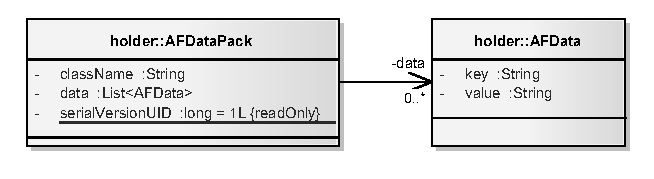
\includegraphics{images/dataPack}
\caption{Třídy, na které jsou převedena všechna data, jenž klient obdrží.}
\label{img:dataPack}
\end{center}
\end{figure}

\subsubsection{Widget builder}
V tabulce \ref{table:widgetBuilders} jsou popsány všechny widget buildery, které je možné použít. Všechny buildery mají společného předka. Abstraktní reprezentace buildera je znázorněna na obrázku \ref{img:abstractBuilder}. Konkrétní instance pak využívá společných metod, jež jsou implementovány v jeho předkovi. Předek umí sestavit placeholder určený k zobrazení výsledku validací, popis ke každé komponentě, nastavit lokalizace, skiny včetně jejich aplikace a přidat validátory na pole. Tato abstraktní třída také umí vygenerovat dummy field, který je vytvořen pouze pokud komponenta dostala list hodnot jichž může nabývat a současně není volba z tohoto listu povinná. Pak je zapotřebí udržovat informaci o tom, že uživatel volbu neučinil. Konkrétní prvky builderu z tabulky \ref{table:widgetBuilders} pak vytváří každý builder sám. 

\begin{lstlisting}[caption={Vytváření vstupního pole builderem.},
label={code:textInputBuilder}, basicstyle=\footnotesize]
public AFSwinxPanel buildComponent(AFFieldInfo field) 
throws IllegalArgumentException, AFSwinxBuildException {
	super.buildBase(field);
	// And input text field
	JTextField textField = new JTextField();
	customizeComponent(textField,field);
	layoutBuilder.addComponent(textField);
	coreComponent = textField;
	// Create panel which holds all necessary informations
	AFSwinxPanel afPanel =
		new AFSwinxPanel(field.getId(), field.getWidgetType(), textField, fieldLabel,
		message);
	// Build layout on that panel
	layoutBuilder.buildLayout(afPanel);
	// Add validations
	super.crateValidators(afPanel, field);
	return afPanel;
}
\end{lstlisting}

Ukázka metody, která vygeneruje vstupní textové pole je znázorněna v části zdrojových kódu \ref{code:textInputBuilder}. Nejprve jsou vytvořeny společné vlastnosti pro všechny buildery. Tyto vlastnosti vytváří abstraktní předek. Poté je vytvořeno vstupné pole a na toto pole je aplikován skin. Komponenta je poté přidána do layout builderu. Následně je vytvořen AFSwinxPanel, jenž nese všechny nezbytné informace o aktuální komponentě. Tento panel je také přidán do layout, který poté vytvoří konečné uspořádání komponent. Nakonec jsou v panelu registrovány všechny validátory, které se postupně spustí v případě odeslání dat, či v případě žádosti o zjištění validnosti formuláře.

\begin{lstlisting}[caption={Vložení dat do vstupního pole vytvořeného builderem.},
label={code:textInputBuilderSetData}, basicstyle=\footnotesize]
public void setData(AFSwinxPanel panel, AFData data) {
	if (panel.getDataHolder() != null && !panel.getDataHolder().isEmpty()) {
		JTextComponent textField = (JTextComponent) panel.getDataHolder().get(0);
		textField.setText(data.getValue());
	}
}
\end{lstlisting}

Jak již bylo zmíněno, builder zná způsob, jakým byly komponenty vytvořeny. Z toho vyplývá, že zná i způsob, jakým jsou reprezentovýny. V případě potřeby vložení dat do textového pole, je potřeba získat builder, který toto pole vytvořil a požádat ho o vložení dat. Ukázka je v části zdrojových kódů \ref{code:textInputBuilderSetData}. Builder nejprve ověří, zdali existují v panelu komponenty. Pokud ano přetypuje je na konkrétní instance, které vytvářel. V tomto případě JTextComponent. Poté jim nastaví data specifickým způsobem pro danou komponentu.

\begin{table}[width=\linewidth]
\begin{center}
\caption{Widget buildery, kterými disponuje klient}
\label{table:widgetBuilders}
\begin{tabular}{|p{4cm}|p{3cm}|p{7cm}|}
\hline
\textbf{Builder} & \textbf{Typ widgetu} & \textbf{Popis} \\
\hline
DateBuilder & 
Calendar & Používá se při reprezentaci datového typu. Umožní uživateli zobrazit date picker, pomocí kterého lze vybrat datum. \\
\hline
DropDownMenuBuilder &
dropDownMenu & Menu, ze kterého lze vybrat jednu z několika voleb. \\
\hline
CheckBoxBuilder & checkBox &
Zaškrtávací políčk či několik zaškrtávacích políček. Záleží, zdali jsou uvedeny možnosti. V případě, že uvedeny nejsou, vytvoří se jedno a pokud je zaškrtnuto je převedeno na hodnotu true. \\
\hline
InputBuilder & textField &
Builder pro textové pole. Nemá žádné výchozí omezení. \\
\hline
LabelBuider & label &
Vypíše pouze textovou hodnotu. Do této komponenty nelze vkládat data ani ji jinak upravovat. \\
\hline
NumberInputBuilder & numberField &
Vytvoří vstupní pole a přidá mu číselnou validaci. \\
\hline
OptionBuilder & option &
Vytvoří skupinu radiobuttonů, z které lze vybrat jednu hodnotu. \\
\hline
PasswordBuilder & password &
Vytvoří vstupní pole, v kterém jsou znaky nahrazeny zástupnými znaky. \\
\hline
TextAreaBuilder & textArea &
Vytvoří vstupní pole pro zadání velkého množství znaků. \\
\hline
\end{tabular}
\end{center}
\end{table}

\subsubsection{Skin}
Widget builder aplikuje na vygenerované komponenty skin. Skin lze nastavit již při získávání formulářového builderu. Skin určuje vzhled konkrétní komponenty. Pomocí skinu lze určit následující vlastnosti.
\begin{enumerate}
\item Barvu, typ fontu, výšku a šířku popisu, který je zobrazen u komponenty.
\item Barvu a typ fontu komponent.
\item Barvu a typ fontu validačních hlášení.
\item Šířku komponent. V případě textových polí i jejich výšku.
\end{enumerate}
Pokud není skin nastaven, potom je použita výchozí implementace, která je součástí frameworku. Vývojář si může definovat vlastní skin a to tak, že buď implementuje rozhraní Skin, nebo využije dědičnost a překryje metody z třídy BaseSkin. Výhodou druhého přístupu je fakt, že vývojář může upravit pouze některé metody a nemusí implementovat všechny, které vyžaduje rozhraní.
\section{Přenos a generování dat klient server}
Formuláře a tabulky jsou vytvářeny k tomu, aby reprezentovali uživateli data v systému. Hlavním úkolem formulářů je také odeslání dat na server. Z předchozích sekcí je již zřejmé, že klientská část aplikace nedisponuje stejnými datovými objekty jako server, ale pouze popisem struktury daného objektu. Tato informace je však dostačující a na jejím základě lze vygenerovat data, která je server schopný přijmout. Přenos probíhá v několika krocích. Tyto kroky zachycuje sekvenční diagram na obrázku \ref{img:sdResealization}. Nejprve je zjištěno, zdali byl při vytváření komponenty specifikován zdroj, na který se mají data odeslat. Před vygenerováním dat, která budou odeslána, je provedena validace. V případě, že je validace úspěšná začnou se generovat data, která budou odeslána. K tomuto účelu slouží třída JSON builder, v případě že server očekává data ve formátu typu JSON. Framework nyní podporuje pouze JSON, nicméně návrh počítá s přidáním dalších datových builderů. Tyto buildery již neparsují data, která jsou uložena v komponentě, neboť za tuto činnost je zodpovědná konkrétní komponenta sama. Komponenta data parsuje z panelů, které si udržuje. Panel má jasně daný klíč, kterým lze určit umístění proměnné v původním objektu. Na základě tohoto klíče je vytvořen nový objekt. Klíč tedy určuje cestu. Pokud je v klíči znak tečky, znamená to, že je potřeba vyhledávat v již existující struktuře další potomky. Pokud v klíči znak tečky není, znamená to, že jsme již na správném místě a objektu, který je reprezentován třídou AFDataHolder, jejíž ukázka je na obrázku \ref{img:afDataHolder}, bude přidána do jeho mapy další proměnná s hodnotou. Kromě klíče je potřeba znát i aktuální data v komponentě. Obdobně jako při vkládání dat do komponenty je i při získávání dat využit konkrétní widget builder, který komponentu sestavil, neboť zná strukturu a způsob, jakým data z komponenty získat. JSON builder tedy dostane objekt, ze kterého může data sestavit. K sestavení dat je využit framework GSON \cite{gson}. Když jsou již data sestavena, postačí je odeslat na konkrétní zdroj, který byl specifikován při vytváření komponenty. Framework toto odeslání provede automaticky.

\begin{figure}[h!]
\begin{center}
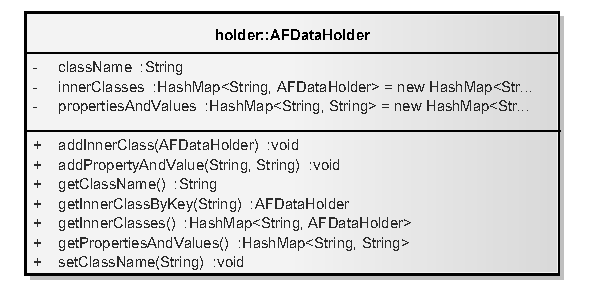
\includegraphics{images/AFDataHolder}
\caption{Třída, která reprezentuje data ve formuláři, na jejím základě je sestaven objekt, který je odeslán na server.}
\label{img:afDataHolder}
\end{center}
\end{figure}

Pokud chce vývojář data odeslat například při kliknutí na tlačítko, musí provést pouze dva kroky. Nejprve musí získat konkrétní formulář, který chce odeslat a poté nad ním zavolat akci sendData. Formulář lze získat z hlavní třídy AFSwinx, na základě jeho identifikátoru, kdekoliv v aplikaci. Žádné další akce nejsou potřeba. Mezi hlavní výhody patří snadná použitelnost formulářů a skutečnost, že je vývojář odstíněn od způsobu jakým se data odesílají. Nevýhodou je, že vývojář nemůže plně kontrolovat odeslání dat, či měnit implementaci odesílání a musí používat pouze metody, které mu framework nabízí.
\section{Lokalizace}
Aplikace mohou mít různé jazykové mutace. Klientská strana frameworku nabízí podporu pro lokalizace. Soubor s lokalizací lze nastavit buď builderu, který staví formulář, nebo třídě, zodpovědné za správu všech vygenerovaných komponent. Pokud je lokalizace nastavena této třídě, pak ji implicitně využijí všechny komponenty, pokud nebude toto nastavení překryto v builderu. Framework disponuje vlastním lokalizačním souborem, ve kterém jsou všechná validační hlášení. Pokud nebyl lokalizační soubor určen, využije se výchozí nastavení, kterým framework disponuje. Toto nastavení se používá pouze pro validační hlášení a pro objekt, který indikuje, že nebyla zvolena žádná hodnota. Hlavním důvodem tohoto chování je fakt, že nelze předpokládat, jaké texty bude chtít klient zobrazit. Pro popisy komponent, které jsou generovány serverem, se používá lokalizační soubor, který specifikoval uživatel. Pokud v něm není hodnota nalezena, použije se hodnota, kterou klient od serveru obdržel. Nemůže se tedy stát, že by byl text během překladu zahozen.
\section{Validace dat a vlastní validátory}
Při odesílání formuláře, je potřeba nejprve provést validace. Důvodem je, že validace omezují model buď na základě datových omezení, nebo na základě business omezení. Pokud server očekává v poli typu integer číslo a obdrží od klienta řetězec, pak dojde k chybě. Úkolem validací je tyto chyby odhalit a poskytnout typovou kontrolu. Framework nenabízí business validace na serverové straně. To znaměná, že se data musí odeslat a pokud dojde k chybě na serveru během zpracování, je o této chybě klient informován. Nicméně z podstaty funkčnosti a návrhu je toto omezení nepřekonatelné, protože klient nemá reference na objekty, na základě kterých byly vygenerovány formuláře či tabulky a také nezná způsob, jakým se s objektem dále pracuje. 
\subsection{Podporované validace}
V současné verzi jsou podporovány validace z tabulky \ref{table:validations}. Všechny validátory jsou registrovány na komponentě až v poslední fázi generování. Výjimku tvoří retype validace, která ke své funkčnosti vyžaduje, aby byl zobrazen druhý identický prvek k widgetu, jenž bude tímto validátorem validován. Tento klon musí být taktéž přidán do aktuálního layoutu a zaregistrován jako komponenta, aby s ním bylo možné pracovat. V panelu je také nastaven speciální klíč a příznak, že se jedná o klon, neboť při generování dat, která budou odeslána na server, nechceme generovat data i z naklonovaného panelu.
\begin{table}[width=\linewidth]
\begin{center}
\caption{Validátory, kterými disponuje klientská část}
\label{table:validations}
\begin{tabular}{|p{4cm}|p{2cm}|p{8cm}|}
\hline
\textbf{Název validátoru} & \textbf{Priorita} & \textbf{Popis funčknosti} \\
\hline
Required & > 2miliony & 
Validátor zjistí, je-li je pole vyplněno, či je vybrána hodnota. Pokud není, je vyhozena výjimka. \\
\hline
NumberValidator & 100 &
Validátor na základě typu widgetu určí, zdali má být v poli integer, double či long. Implicitní hodnota je integer. Poté získá aktuální hodnotu. Pokud hodnota nevyhovuje datovému typu, je vyhozena výjimka. \\
\hline
MinAndMaxValue & 50 &
Validátor porovná aktuální hodnotu s minimální a maximální hodnotou. Pokud aktuální hodnota nevyhovuje, je vyhozena výjimka. \\
\hline
MinAndMaxLength & 70 &
Validátor porovná počet znaků aktuální hodnoty s minimem a maximem, pokud aktuální hodnota nevyhovuje, je vyhozena výjimka. \\
\hline
Retype & 10 &
Validátor zjistí, zdali se hodnota v aktuálním poli shoduje s hodnotou v jiném poli. Pokud hodnoty nevyhovují, je vyhozena výjimka. \\
\hline
\end{tabular}
\end{center}
\end{table}

\subsection{Vyhodnocení validací}
Validace musí být vyhodnocovány v určitém pořadí. Nejprve je třeba vyhodnotit, má-li být pole vyplněné a až poté vyhodnocovat, jsou-li v poli pouze číselné hodnoty. Validátory jsou proto registrovány do prioritní fronty, kterou panel disponuje. U každého validátoru je nastavena jeho priorita, která určuje pořadí, v jakém budou validace ověřovány. Validaci vyvolává klient, pokud chce znát validitu formuláře, či framework automaticky v případě, že je požadováno odeslání dat na server. Validátory jsou řízeny výjimkami. Pokud validace není splněna, je vyhozena výjimka. V případě výjimky zareaguje framework tak, že ji odchytí a zobrazí její textovou reprezentaci u příslušného políčka, poté pokračuje s vyhodnocováním. Formulář, je tedy vždy celý validován. Klient si může doimplementovat vlastní validátor a následně ho zaregistorvat ke konkrétnímu panelu, který lze získat z vygenerovaného formuláře. Opět má klient dvě možnosti jak validátor vytvořit. Doporučeným způsobem je dědit od třídy AFBaseValidator a překrýt metodu validate. Tyto třídy jsou znázorněny na obrázku \ref{img:validationModel}.
\begin{figure}[h!]
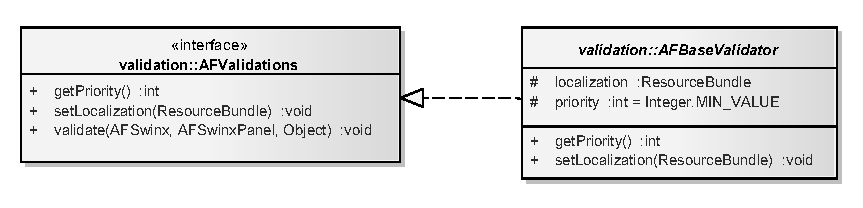
\includegraphics{images/validationModel}
\caption{Abstraktní třídy validátorů, které lze použít k implementaci vlastního validátoru.}
\label{img:validationModel}
\end{figure}

\section{Layouty}
Komponenty v rámci formuláře musí být uspořádany tak, aby byl formulář dobře ovladatelný. Způsob jakým toho lze dosáhnout je specifický pro danou technologii. Nicméně server generuje stále stejné definice bez ohledu na technologii, kterou používá klient. Uspořádání komponent je definováno pomocí osy, ve které jsou prvky zobrazovány počtem sloupců a pozicí popisu komponenty v případě, že jde o konkrétní aktivní prvky formuláře. V případě, že jde o layout formuláře, není popis komponenty uveden. Definice layoutu může nabývat těchto hodnot:
\begin{enumerate}
\item layoutOrientation - orientace layoutu. Nabývá těchto hodnot osa X či Y (AxisX, AxisY)
\item layout - typ layoutu. Nabývá těchto hodnot: jednosloupcový či dvousloupcový (OneColumnLayout, TwoColumnsLayout)
\item labelPossiton - pozice popisu komponenty. Nabývá těchto hodnot před, za, není. (Before, After, None)
\end{enumerate}
Layout je tedy potřeba na klientovi správně interpretovat a na základě jeho specifikace zobrazit komponenty v definované mřížce. Určení absolutní pozice komponenty ve formuláří není možné. Nicméně lze ovlivňovat pořadí, ve kterém jsou komponenty zobrazovány. Toto pořadí určuje server a klient zobrazuje komponenty v pořadí, v jakém je obdržel. 
\subsection{Layout builder}
Ve Swingu je několik layoutů, které jsou jeho součástí a pak samozřejmě existují knihovny, které poskytují speciálně vytvořené a upravené layouty. Jedním z nejvíc komplexních a flexibilních layoutů je GridBagLayout \cite{gridBagLayout}. Výhodou je, že ne všechny komponenty musí mít stejnou výšku, lze tedy vynutit specifické nastavení a docílit tak požadovaného vzhledu. Nevýhodou je složitost tohoto nastavení. Aby bylo možné dosáhnout požadovaného vzhledu, je potřeba kombinovat Swingové layouty. Framework disponuje svým vlastním implicitním builderem, který vytváří GridBagLayout složený z BoxLayoutu. Tento builder umí vytvářet layouty pro jednotlivé komponenty formuláře, ale i pro celý formulář. Nejprve je builder inicializován, poté jsou definovány komponenty, ze kterých je potřeba layout poskládat a následně je layout vytvořen. Tento objekt je reprezentován panelem, jenž lze zobrazit. V tomto panelu jsou již všechny komponenty vykresleny a uspořádány v požadovaném pořadí. 

Layout builder, určený k uspořádání prvků v rámci komponenty je využit v konkrétním widget builderu, který má znalost o tom, jaké prvky je potřeba přidat. Například vstupní textové pole má pouze tři prvky. Jsou jimi popis, samotné vstupní pole a placeholder určený k zobrazení validačního hlášení. Oproti tomu zaškrtávací políčka mají více komponent, neboť lze mít více zaškrtávacích políček, které mohou mít svoje popisy. Výhodou následujícího využití je v budoucnu možnost specifické implementace layoutu v závislosti na typu komponenty. Layout builder, určený k sestavení formuláře je využit ve formulářovém builderu. Tento builder má znalost, obdobně jako widget builder, o všech komponentách formuláře a jejich umístění. 

\section{Bezpečnost}
Součástí každé aplikace je i zabezpečení. Na oblast bezpečnosti lze nahlížet z několika aspektů. Jedním z těchto aspektů je šifrování dat a ověření, komunikuje-li klient opravdu se správným serverem. Druhým aspektem je bezpečnost v rámci aplikace. S tím je spojená autentizace a autorizace zdrojů. Framework neposkytuje komplexní zabezpečení, ale v některých ohledech nabízí nástroje, kterými toho lze dosáhnout.

\subsection{Přenos dat}
Klient může specifikovat protokol, s jehož pomocí, klient komunikuje se serverem. Framework nabízí protokoly HTTP nebo HTTPS \cite{https}. Výhodou HTTPS je HTTP protokol, který využívá SSL. Princip přenosu data je obdobný jako v případě HTTP. Nejprve klient vytvoří připojení na server a vyžádá si připojení přes SSL a poté pošle HTTP request pomocí SSL. HTTPS připojení vyžaduje svůj vlastní port. 

Pokud chce uživatel využít protokolu HTTPS, tak je potřeba framework nastavit. Nastavení musí být provedeno na konkrétním datovém zdroji, který je specifikován pomocí XML. S ohledem na uživatele byla přidána funkcionalita, která umí request pro HTTPS sestavit automaticky. Uživatel tedy pouze, v XML souboru se zdroji, uvede jako typ protokolu HTTPS a port, na kterém server umožňuje HTTPS požadavek přijmout. Pokud je certifikát serveru nevalidní, pak request pomocí HTTPS nelze provést.

\subsection{Autentizace a autorizace}
V netriviálních aplikacích je potřeba ověři,t zná-li systém uživatele, a zdali má uživatel právo provádět specifické akce. Ověření uživatele je autentizace. Výsledkem procesu autentizace je informace, jestli uživatele známe, tedy může-li se uživatel přihlásit do aplikace. Autorizace již ověřuje, jestli má přihlášený uživatel práva provádět specifické akce. Obvykle existuje tzv: Security Context, který umí ověřit, je-li uživatel v určité roli. Vzhledem k tomu, že framework je navržen tak, aby komunikoval se serverem pomocí HTTP či HTTPS, tak jsou možnosti autentizace a autorizace omezenější. Je potřeba umět na server odeslat uživatelské jméno a heslo. K tomuto účelu lze použít autorizaci typu basic. Klientská strana disponuje podporou pro tento typ autorizace. Obdobným způsobem jako v případě HTTPS, lze určit metodu, uživatelské jméno a heslo v XML souboru, který specifikuje připojení. Aby se hodnoty daly měnit za chodu aplikace, lze využít EL a konkrétní hodnoty nastavit až při generování definice zdrojů v klientské části. Na serverové straně lze vyřešit zabezpečení způsobem, jaký si vývojář sám zvolí. Framework AspectFaces \cite{aspectFaces}, který je použit ke generování dat, disponuje anotací @UiUserRoles, pomocí které lze určit, při jakých uživatelských rolích bude proměná inspektována. Konkrétní roli uživatele je pak potřeba určit v kontextu. Zabezpečení pomocí oAuth není v současné verzi možné, ale framework umožňuje v hlavičce requestu odestlat jakýkoliv parameter. Například synchronizační token. 

\section{Porovnání přístupů}
Při vytváření prezentační vrstvy dochází opakování kódů, což je v rozporu s jedním z principů vývoje softwaru. Tento prinicip se nazývá DRY. Do not repeat yourself. Bohužel nelze tento princip dodržovat striktně, neboť pokud vývojář chce zobrazit aktivní prvek, vždy musí vytvořit instanci určité komponenty či komponentu specifikovat. Formuláře obvykle mají několik komponent a každá z nich bude mít popis, aktivní prvek, validační hlášení a validaci jejíž logika musí být napsána. Dále je potřeba takto vygenerovaný formulář naplit a poté z něj získat data. Toto všechno musí vývojář naprogramovat. Kromě toho je potřeba také umístit komponenty do vhodného layoutu a zohlednit bezpečnost. I přes použití různých návrhových zdrojů, jako je například MVC \cite{fowler} má výsledný kód mnoho řádků, které se v případě změny musí revidovat. Pokud formulář získává data ze serveru, musí být doimplementovány připojení na server, způsob získání dat, jejich uložení, reprezentace těchto dat a zpětné odeslání na server. Výhodou však zůstává, že má vývojář plnou kontrolu nad generovanou prezentační vrstvou a implementuje klienta vůči API na serveru, které se nemusí upravovat.

Pokud jsou komponenty generovány frameworkem, nemá nad nimi vývojář plnou kontrolu. Musí pracovat s API, které framework poskytuje a nemůže si komponenty nastavovat jinak, než framework dovolujte a je potřeba na server umístit zdroj, který bude generovat definice. Výhody jsou však mnohem větší. Není potřeba implementovat připojení na server a základní autorizace. O reprezentaci dat se framework také postará, stejně tak jako o získání dat a vygenerování aktivních komponent dle serverové specifikace. Validátory a jejich logika je také součástí takto vygenerovaných komponent. Prezentační vrstva reaguje pružně na změny datových typů a uživatelských rolí. Důvodem je přístup k vytváření uživatelského rozhraní, při kterém se vždy zohledňují aspekty. Jedním z aspektů jsou komponenty, které jsou uživateli zobrazeny, dalším jsou způsoby, jak je sestavit, získat z nich data či do komponent data vložit. Způsoby validace a způsob jakým klient se serverem komunikuje. Jednou z největších výhod je ale fakt, že lze měnit prezentační vrstvu klienta přímou změnou na serveru. Ve většině případů neznamená změnový požadavek na klientskou prezentační vrstvu nutnost distribuovat novou verzi.

